% Unnumbered commutative diagram from original page 40.
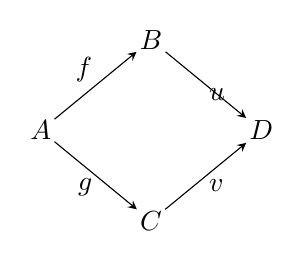
\begin{tikzpicture}[
  baseline=(current bounding box.center),
  every node/.style={inner sep=1pt},
  every path/.style={->,>=stealth}
]
  \node (A) at (0,0) {$A$};
  \node (B) at (1.4,1.15) {$B$};
  \node (C) at (1.4,-1.15) {$C$};
  \node (D) at (2.8,0) {$D$};

  \draw (A) -- node[above left] {$f$} (B);
  \draw (A) -- node[below left] {$g$} (C);
  \draw (B) -- node[below right] {$u$} (D);
  \draw (C) -- node[below right] {$v$} (D);
\end{tikzpicture}
